% The beamer class automatically loads some other LATEX packages, including
% xcolor, amsmath, amsthm, calc, geometry, hyperref, extsizes.
% color predefined:red, blue, green, cyan, magenta, yellow, black, darkgray, gray,
% lightgray, orange, violet, purple, brown
% \documentclass[11pt]{beamer}
\documentclass[pdf]{beamer}
% aspectratio=1610
% default font size 11pt;8pt, 9pt, 10pt, 11pt, 12pt, 14pt, 17pt, 20pt
% used to print as article
% \documentclass[]{article}
% \usepackage{beamerarticle}

% Antibes, Bergen, Berkeley, Berlin, Boadilla, Copenhagen, Darmstadt, Dresden,
% Frankfurt, Goettingen, Hannover, Ilmenau, Juanlespins, Madrid, Malmoe,
% Marburg, Montpellier, Paloalto, Pittsburgh, Rochester, Singapore, Warsaw
% \usetheme[compress]{Singapore} %title at the top-middle
% \usecolortheme{freewilly}
\usetheme{Boadilla}
% \beamertemplatetransparentcoveredhigh
% \beamertemplatetransparentcovereddynamicmedium

\usepackage[T1]{fontenc}
% \mode<article> % 仅应用于article版本
% {
% \usepackage{beamerbasearticle}
% \usepackage{fullpage}
% \usepackage{hyperref}
% }

%   font theme
%   \usefonttheme[onlymath]{serif}
%   \usefonttheme{structureitalicserif}
%   \usefonttheme{structurebold}
%   \usefonttheme{structuresmallcapsserif}
%   \usepackage{lucidaso} % Lucida Bright (SO Version)
\usefonttheme[onlymath]{serif}
% \usepackage[small]{eulervm} % Euler VM for math font
% \usepackage{helvet}


% color themes:albatross crane beetle dove fly seagull wolverine beaver
% \usecolortheme{fly}
% Outer color themes:whale, seahorse, dolphin
\usecolortheme{whale}
% Inner color themes: lily, orchid,rose
\usecolortheme{orchid}

% rectangles circles inmargin rounded
\useinnertheme{rectangles}
% \useinnertheme[shadow]{rounded} % 对 box 的设置: 圆角、有阴影.
% infolines miniframes shadow sidebar c smoothtree split tree progressbar
\useoutertheme{progressbar}

% define colors
% \setbeamercolor{uppercol}{fg=white,bg=blue}%
\setbeamercolor{lowercol}{fg=black,bg=gray}%
\xdefinecolor{lavendar}{rgb}{0.8,0.6,1}
\xdefinecolor{olive}{cmyk}{0.64,0,0.95,0.4}
\colorlet{structure}{green!60!black}
% redefine structure color
% \usecolortheme[named=yellow]{structure}
% redefine alert color
% \setbeamercolor{alerted text}{fg=cyan}

\setbeamertemplate{headline}[default]

% \beamertemplateshadingbackground{blue!5}{yellow!10}
% \setbeamertemplate{background canvas}[vertical
% shading][top=blue!30,bottom=white,middle=blue!20,midpoint=.4]
% \setbeamertemplate{sidebar canvas
% left}[horizontal shading][left=white!40!black,right=black]
% \setbeamertemplate{navigation symbols}{}
\mode<beamer>{\setbeamertemplate{blocks}[rounded][shadow=true]}
% transparent,highly dynamic,dynamic,
\setbeamercovered{invisible}
\setbeamercolor{body}{fg=blue!80, bg=black!20}
\setbeamercolor{head}{fg=blue,bg=blue!30}

\setbeamerfont{title}{shape=\slshape,family=\ttfamily,series=\bfseries}

\beamertemplateballitem

\usepackage{wasysym}
\usepackage{pifont}
% \usepackage{textcomp}

% \usepackage{pgf,pgfarrows,pgfnodes,pgfautomata,pgfheaps}


\usepackage{graphicx}

% shadowbox,fbox,Ovalbox,ovalbox,doublebox
\usepackage{fancybox}
\usepackage{fancyvrb}

\usepackage{multimedia}
\usepackage{listings}
\usepackage{boxedminipage}
% \usepackage{babel}
% \usepackage{enumitem}
\usepackage{array}

\lstset{
  % 行号
  numbers=left,
  % 背景框
  framexleftmargin=10mm,
  frame=none,
  captionpos=b,
  % 背景色
  % backgroundcolor=\color[rgb]{1,1,0.76},
  % backgroundcolor=\color[RGB]{245,245,244},
  % 样式
  keywordstyle=\bf\color{blue},
  identifierstyle=\bf\color{black!90},
  numberstyle=\color[RGB]{0,192,192}\tiny,
  commentstyle=\it\color[RGB]{0,96,96},
  stringstyle=\rmfamily\slshape\color[RGB]{128,0,0},
  % 显示空格
  showstringspaces=false
}


\title[prune]{LLVM based Program Pruning against Special Concerns}
\author{Hongxu Chen}
\subject{Test Generation, Regression Testing}
\date[date]{\today}

\AtBeginSection[]{
  \frame<handout:0>{
    \frametitle{Outline}
    \tableofcontents[current,currentsubsection,shaded]
  }
  \addtocounter{framenumber}{-1}%
}

\hypersetup{pdfpagemode={FullScreen}}
% \hypersetup{pdfstartview={FitH}}

\makeatletter
\newenvironment{CenteredBox}{%
  \begin{Sbox}}{% Save the content in a box
  \end{Sbox}\centerline{\parbox{\wd\@Sbox}{\TheSbox}}}% And output it centered
\makeatother

\newenvironment<>{varblock}[2][\textwidth]{%
  \setlength{\textwidth}{#1}
  \begin{actionenv}#3%
    \def\insertblocktitle{#2}%
    \par%
    \usebeamertemplate{block begin}}
  {\par%
    \usebeamertemplate{block end}%
  \end{actionenv}}

\begin{document}
\frame{\titlepage}
\frame{\maketitle}

\part{Pruning}
% \frame{\partpage}

\section{Motivation}

\begin{frame}[<+-|alert@+>]
  \frametitle{\secname}
  \begin{itemize}
  \item Accurately pruning unrelated snippets w.r.t concerns can:
    \begin{enumerate}
    \item help program understanding
    \item help to generate regression testing
    \item avoid unnecessary path constraints solving in symbolic execution
      \begin{itemize}
      \item[\ding{43}] Focus on a specific \alert{assert} error
      \item[\ding{43}] Less code $\Rightarrow$ less time to locate a special bug
      \end{itemize}
    \end{enumerate}
    \vskip18pt
  \item For a given \textcolor{blue}{program point} and an \textcolor{blue}{entry function}:
    \begin{itemize}
    \item find emph possible paths that \textcolor{blue}{reaches} the point
    \item get the statements \textcolor{blue}{affecting} the point
    \end{itemize}
  \end{itemize}
\end{frame}

\section{Approach}

\begin{frame}
  \frametitle{Requirements}
  \begin{itemize}
  \item Pruning should be \alert{conservative} \pause
  \item Prune as many instructions as possible \pause
  \item The remaing snippets should be \alert{executable}
  \end{itemize}
\end{frame}


\begin{frame}
  \frametitle{\secname}
  \begin{enumerate}
  \item Build points-to set for the given translation unit $\Leftarrow$\textcolor{red}{program point}
  \item Build accurate callgraph $\Leftarrow$ \textcolor{blue}{points-to}
  \item Eliminate un-called functions $\Leftarrow$ \textcolor{red}{entry function}, \textcolor{blue}{callgraph}
  \item Build modification info $\Leftarrow$ \textcolor{cyan}{points-to}
  \item Inter-procedural Reachability Analysis $\Leftarrow$ \textcolor{cyan}{un-called function elimination}
  \item Inter-procedural Slicing $\Leftarrow$ \textcolor{cyan}{un-called function elimination}, \textcolor{cyan}{modify set}, \textcolor{cyan}{callgraph}, \textcolor{cyan}{points-to}
  \end{enumerate}
\end{frame}

\section{Issues and Solutions}

\begin{frame}[containsverbatim]
  \frametitle{Andersen's Inaccruacy}
  \centering{\begin{block}{}
      \begin{CenteredBox}
        {{\tiny
            \begin{lstlisting}[language={[ANSI]C}]
              void foo(void) {
                int a, i, j, k;
                int *p;
                if (a < 0) {
                  p = &i;
                  *p = 3;
                } else if (a > 0) {
                  p = &j;
                  *p = 3;
                  assert(j > 0); // <= interest point
                }
                p = &k;
                *p = 3;
              }
            \end{lstlisting}}}
      \end{CenteredBox}
    \end{block}}
\end{frame}

\begin{frame}[containsverbatim]
  \frametitle{CallGraph Example}
  \begin{columns}

    \column{.45\textwidth}
    {{\tiny{
          \begin{lstlisting}[language={[ANSI]C}]
  int dec(int i) {
    return i - 1;
  }
  
  unsigned long func1(int i) {
    if (i == 0) return 1;
    return func1(dec(i)) * i;
  }
  
  unsigned long func2(int i) {
    return i * 0;
  }
  
  unsigned long (*pF)(int) = func1;
  
  int getNextRandomValue(void) {
    return rand() % 10;
  }

          \end{lstlisting}
        }}
    }

    \column{.45\textwidth}
    {{\tiny{
        \begin{lstlisting}[language={[ANSI]C}]
  void populate_array(int *array,
  size_t arraySize,
  int (*getNextValue)(void)) {
    for (unsigned i = 0;
    i < arraySize; i++)
    array[i] = getNextValue();
  }
  
  int main(void) {
    int i = 3;
    int myarray[10];
    if (i < 3) {
      pF = func1;
    } else {
      pF = func2;
    }
    pF(getNextRandomValue());
    populate_array(myarray, 10,
    getNextRandomValue);
  }
        \end{lstlisting}
      }}}
  \end{columns}

  % \centering\shadowbox{A Simple Program}

\end{frame}

\begin{frame}
  \frametitle{CallGraph Comparison}
  \begin{columns}
    \column{.45\textwidth}
    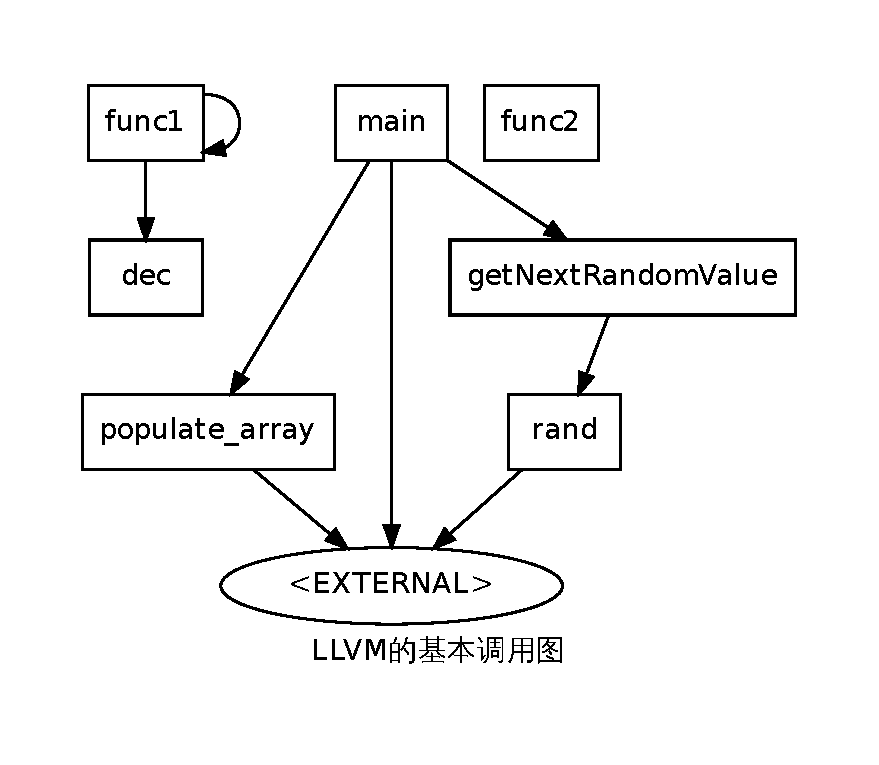
\includegraphics[width=\textwidth]{res/cg_llvm.pdf}
    \column{.45\textwidth}
    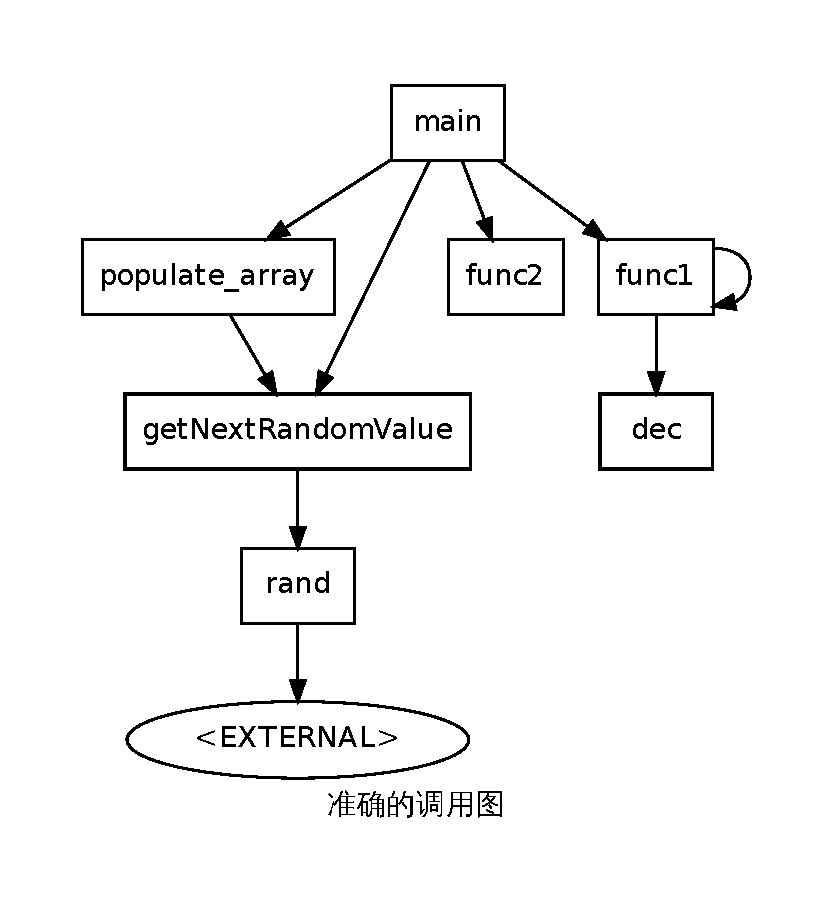
\includegraphics[width=\textwidth]{res/cg.pdf}
  \end{columns}
\end{frame}

\begin{frame}[containsverbatim]
  \frametitle{Inter-procedural Reachability}
  \begin{columns}
    \column{.45\textwidth}
  \begin{CenteredBox}
    {\tiny{
        \begin{lstlisting}[ basicstyle=\ttfamily\bfseries, language={[ANSI]C}]
          int foo(int i) {
            if (i < 0) {
              assert(0); // <=
              return -i;
            } else {
              return i;
            }
          }

          int foo1(int i) { return foo(i); }

          int foo2(int i) { return foo(i); }

          int main(void) {
            int i = -1;
            // foo1(i);
            foo2(-i);
            foo(i);
            return 0;
          }

        \end{lstlisting}
      }}
  \end{CenteredBox}
  \column{.45\textwidth}
    \begin{Verbatim}[commandchars=\\\{\}, fontsize=\tiny]

\textcolor{black}{define i32 @foo(i32 %i) [}
\textcolor{black}{entry:}
\textcolor{black}{  %cmp = icmp slt i32 %i, 0}
\textcolor{black}{  br i1 %cmp, label %if.then, label %if.else}

\textcolor{black}{if.then:}
\textcolor{cyan}{  call void @__assert_fail(<...>)}
\textcolor{blue}{  unreachable}

\textcolor{black}{if.else:}
\textcolor{blue}{  ret i32 %i /// <=}

\textcolor{black}{declare void @__assert_fail(i8*, i8*, i32, i8*)}

\textcolor{blue}{define i32 @foo1(i32 %i) [}
\textcolor{blue}{entry:}
\textcolor{blue}{  %call = call i32 @foo(i32 %i)}
\textcolor{blue}{  ret i32 %call}
\textcolor{blue}{]}

\textcolor{black}{define i32 @foo2(i32 %i) [}
\textcolor{black}{entry:}
\textcolor{black}{  %call = call i32 @foo(i32 %i)}
\textcolor{black}{  ret i32 %call /// <=}
\textcolor{black}{]}

\textcolor{black}{define i32 @main() [}
\textcolor{black}{entry:}
\textcolor{black}{  %call = call i32 @foo2(i32 0)}
\textcolor{black}{  %call1 = call i32 @foo(i32 0)}
\textcolor{blue}{  ret i32 0 /// <= }
\textcolor{black}{]}
\end{Verbatim}

\end{columns}
\end{frame}

\appendix
\newcount\opaqueness
\begin{frame}
  \itshape
  \animate<1-5>
  \Large

  \only<1-5>{
    \animatevalue<1-5>{\opaqueness}{20}{100}
    \begin{colormixin}{\the\opaqueness!averagebackgroundcolor}
      \begin{centering}
        \Huge{\color{cyan!60!black} Thank You} \smiley\par
      \end{centering}
    \end{colormixin}
  }
\end{frame}

\end{document}
